\documentclass[11pt,a4paper]{article}

% Typeface: XeLaTeX with Latin Modern Roman (fontspec default)
\usepackage{fontspec}
\usepackage{polyglossia}
\setdefaultlanguage[variant=british]{english}

% Page: the measures of the note template (A4, 11 pt, 4.5 cm side margins, header and page count)
\usepackage[a4paper,left=4.5cm,right=4.5cm,top=4.5cm,bottom=4.1cm,headheight=14pt,headsep=0.55cm,
  footskip=0.55cm]{geometry}
\linespread{0.946}
\usepackage{fancyhdr}
\usepackage{lastpage}
\pagestyle{fancy}
\fancyhf{}
\fancyhead[L]{\small\textbf{PROJECT NOTE} $|$ USD/TRY trend}
\fancyhead[R]{\small\textbf{Compiled on:} \notedate}
\fancyfoot[C]{\small\thepage\,/\,\pageref{LastPage}}
\renewcommand{\headrulewidth}{0.4pt}

\usepackage{microtype}
\usepackage{amsmath,amssymb}
\usepackage{booktabs,array,tabularx}
\usepackage{graphicx}
\usepackage{enumitem}
\setlist{noitemsep, topsep=3pt, leftmargin=*}
\usepackage{xcolor}
\definecolor{secblue}{HTML}{1F3A5F}
\definecolor{boxback}{HTML}{EEF2F6}
\definecolor{mark}{HTML}{9B2226}
\definecolor{hl}{HTML}{FFF36B}
\makeatletter
\def\hl#1{{\setlength{\fboxsep}{0.4pt}\hl@word#1 \@nil}}
\def\hl@word#1 #2\@nil{\colorbox{hl}{\strut #1}%
  \if\relax\detokenize{#2}\relax\else\colorbox{hl}{\strut\ }\allowbreak\hl@word#2\@nil\fi}
\makeatother
\usepackage{titlesec}
\titleformat{\section}{\color{secblue}\bfseries\normalsize}{\thesection.}{0.4em}{}
\titlespacing*{\section}{0pt}{10pt}{4pt}
\usepackage[font=small,labelfont=bf,labelsep=period,skip=4pt]{caption}
\usepackage[bottom]{footmisc}

\setlength{\parindent}{0pt}
\setlength{\parskip}{5pt}
\setlength{\textfloatsep}{10pt}
\emergencystretch=3em

\newcommand{\notedate}{\number\day\space\ifcase\month\or January\or February\or March\or April\or May\or June\or
  July\or August\or September\or October\or November\or December\fi\space\number\year}

\newcommand{\Months}{177}
\newcommand{\FirstMonth}{2012-01}
\newcommand{\LastMonth}{2026-09}
\newcommand{\UsdFirst}{1.84}
\newcommand{\UsdLast}{48.56}
\newcommand{\UsdRatio}{26.3}
\newcommand{\UsdGrowth}{1.86}
\newcommand{\UsdTrendB}{2.09}
\newcommand{\UsdRTwo}{0.960}
\newcommand{\UsdDW}{0.033}
\newcommand{\UsdResidRho}{0.98}
\newcommand{\UsdResidMin}{$-$43}
\newcommand{\UsdResidMax}{50}
\newcommand{\UsdAdfLevel}{0.46}
\newcommand{\UsdPF}{0.86}
\newcommand{\UsdPKW}{0.65}
\newcommand{\EurFirst}{2.38}
\newcommand{\EurLast}{55.96}
\newcommand{\EurRatio}{23.5}
\newcommand{\EurGrowth}{1.79}
\newcommand{\EurTrendB}{2.00}
\newcommand{\EurRTwo}{0.950}
\newcommand{\EurDW}{0.029}
\newcommand{\EurResidRho}{0.99}
\newcommand{\EurResidMin}{$-$39}
\newcommand{\EurResidMax}{53}
\newcommand{\EurAdfLevel}{0.52}
\newcommand{\EurPF}{0.60}
\newcommand{\EurPKW}{0.63}
\newcommand{\TestFirst}{2021-10}
\newcommand{\TestLast}{2026-09}
\newcommand{\UsdDriftHOne}{4.5}
\newcommand{\UsdDriftHTwelve}{25.2}
\newcommand{\UsdExpHOne}{36.0}
\newcommand{\UsdExpHTwelve}{47.3}
\newcommand{\UsdRWHOne}{5.2}
\newcommand{\UsdRWHTwelve}{39.2}
\newcommand{\UsdDampedHOne}{5.2}
\newcommand{\UsdDampedHTwelve}{28.2}
\newcommand{\UsdHWHOne}{5.8}
\newcommand{\UsdHWHTwelve}{42.7}
\newcommand{\EurDriftHOne}{4.6}
\newcommand{\EurDriftHTwelve}{22.3}
\newcommand{\EurExpHOne}{37.9}
\newcommand{\EurExpHTwelve}{49.9}
\newcommand{\EurRWHOne}{5.3}
\newcommand{\EurRWHTwelve}{37.0}
\newcommand{\EurDampedHOne}{4.6}
\newcommand{\EurDampedHTwelve}{21.9}
\newcommand{\EurHWHOne}{4.9}
\newcommand{\EurHWHTwelve}{21.8}


\begin{document}

\vspace*{14pt}
\begin{tabular}{@{}p{2.35cm}@{}p{\dimexpr\textwidth-2.35cm}@{}}
\textbf{TITLE:} & \textbf{\large The trend of USD/TRY and EUR/TRY: moving averages, an exponential trend and exponential smoothing, checked on new months}\\[3pt]
\textbf{SUBJECT:} & Aim, method and results of version 2 of the \texttt{USD\_Exp\_MA\_TrendAnalysis} repository\\[3pt]
\textbf{AUTHOR:} & Muhammed İkbal Yılmaz (myucanlar@gmail.com)
\end{tabular}

\vspace{8pt}
\textbf{Key finding.} Both rates grew by about 2\% a month, and an exponential trend fits them with $R^2$ of \UsdRTwo{} (USD) and
\EurRTwo{} (EUR); \hl{yet the trend leaves deviations that persist for years, and its forecast errors one month ahead are about eight times those of a random walk with drift.} The trend of the exchange rate is stochastic, there is no monthly seasonality, and no smoothing method beats
the drift by more than half a point at any horizon.

\section{Data and design}

Monthly averages of the CBRT indicative buying and selling rates (EVDS, TP.DK.USD.A/S.YTL and TP.DK.EUR.A/S.YTL), \FirstMonth{} to
\LastMonth{} (\Months{} months), downloaded on 26 October 2026. As in version 1, the rate is the mean of the buying and selling rate.
USD/TRY rose from \UsdFirst{} to \UsdLast{} (a factor of \UsdRatio{}), EUR/TRY from \EurFirst{} to \EurLast{} (\EurRatio{}); the mean
monthly change was \UsdGrowth{}\% and \EurGrowth{}\%. All series are $y_t = 100\log(\text{rate}_t)$, so that changes are in per cent.

\section{Trend: moving averages and the exponential trend (Figure 1)}

\textbf{Method.} The $2\times12$ centred moving average,
$\hat T_t = \tfrac{1}{24}y_{t-6} + \tfrac{1}{12}\sum_{j=-5}^{5} y_{t+j} + \tfrac{1}{24}y_{t+6}$, removes any fixed 12-month
pattern and is centred on $t$; it is missing for the first and last six months. (The 3-month average of version 1,
$\tfrac13(y_t+y_{t-1}+y_{t-2})$, is trailing: it is centred on $t-1$, one month behind.) The exponential trend is
$y_t = a + bt + u_t$ by OLS.

\textbf{Finding.} $\hat b$ = \UsdTrendB{}\% a month for USD and \EurTrendB{}\% for EUR. The residuals range from \UsdResidMin{} to
\UsdResidMax{}\% (USD), their first autocorrelation is \UsdResidRho{} and the Durbin--Watson statistic \UsdDW{} (EUR: \EurDW{}): the
series stays above or below the trend for years. The ADF test does not reject a unit root in $y_t$ around a linear trend
($p$ = \UsdAdfLevel{} and \EurAdfLevel{}) and rejects it in $\Delta y_t$ ($p < 0.001$).

\textbf{Interpretation.} A high $R^2$ here measures the common upward drift of $y_t$ and $t$, not the quality of the trend; with a unit
root the deviations from a fixed line do not die out.

\begin{figure}[t]
\centering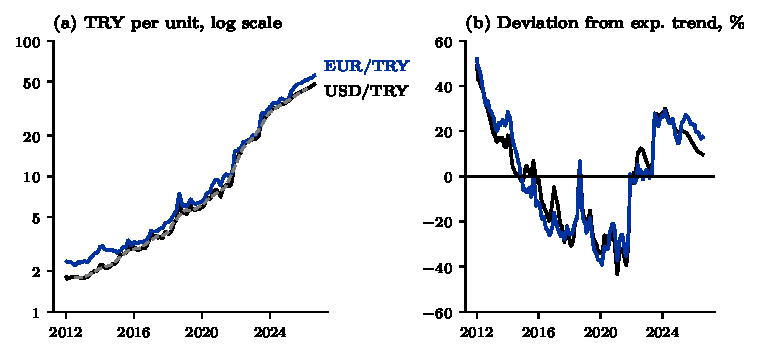
\includegraphics[width=\textwidth]{../figures/fig1_trend.pdf}
\caption{(a) USD/TRY (black) and EUR/TRY (blue), TRY per unit, log scale; dashed grey: $2\times12$ centred moving average of USD/TRY.
(b) Deviation of $y_t$ from the fitted exponential trend, per cent.}
\end{figure}

\section{Seasonality (Figure 2)}

\textbf{Method.} The monthly change $\Delta y_t$ is regressed on a constant and 11 month dummies (F test), and compared across the 12
calendar months with the Kruskal--Wallis test.

\textbf{Finding.} Neither test finds a monthly pattern: $p$ = \UsdPF{} and \UsdPKW{} (USD), \EurPF{} and \EurPKW{} (EUR). A seasonal
component (Holt--Winters, seasonal decomposition) has nothing to estimate.

\begin{figure}[t]
\centering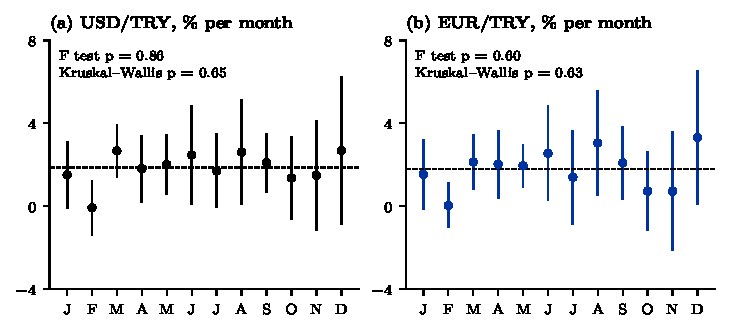
\includegraphics[width=\textwidth]{../figures/fig2_seasonality.pdf}
\caption{Mean monthly change of USD/TRY (a) and EUR/TRY (b) in each calendar month, with 95\% intervals ($\pm1.96$ standard errors);
dashed: mean over all months.}
\end{figure}

\section{Forecasts on new months (Table 1, Figure 3)}

\textbf{Method.} For each month from \TestFirst{} to \TestLast{} (60 months), every method is fitted on the earlier months only and
forecasts 1, 3 and 12 months ahead: random walk ($\hat y_{t+h}=y_t$), random walk with drift ($\hat y_{t+h}=y_t+h\bar{\Delta y}$),
exponential trend, simple exponential smoothing, Holt, damped Holt and Holt--Winters (additive, 12 months). Accuracy is the root mean
squared error (RMSE) in per cent.

\textbf{Finding.} The exponential trend has the largest errors at every horizon: \UsdExpHOne{}\% one month ahead for USD against
\UsdDriftHOne{}\% for the drift. Simple exponential smoothing equals the random walk (the fitted smoothing weight is 1). For USD the drift
is the most accurate at every horizon (\UsdDriftHTwelve{}\% at 12 months); for EUR the drift, damped Holt and Holt--Winters are within
half a point of one another at 12 months (\EurDriftHTwelve{}\%, \EurDampedHTwelve{}\% and \EurHWHTwelve{}\%).

\begin{table}[t]
\centering\small
\caption{RMSE of forecasts on the 60 months from \TestFirst{} to \TestLast{}, per cent of the rate.}
\begin{tabular}{@{}lrrrrrr@{}}
\toprule
 & \multicolumn{3}{c}{USD/TRY} & \multicolumn{3}{c}{EUR/TRY}\\
\cmidrule(lr){2-4}\cmidrule(l){5-7}
Method & 1 m & 3 m & 12 m & 1 m & 3 m & 12 m\\
\midrule
Random walk & 5.2 & 12.6 & 39.2 & 5.3 & 12.4 & 37.0 \\
Random walk with drift & 4.5 & 10.1 & 25.2 & 4.6 & 9.9 & 22.3 \\
Exponential trend & 36.0 & 38.1 & 47.3 & 37.9 & 40.1 & 49.9 \\
Simple exponential smoothing & 5.2 & 12.6 & 39.2 & 5.3 & 12.4 & 37.0 \\
Holt & 5.5 & 13.4 & 42.4 & 4.7 & 10.2 & 23.3 \\
Damped Holt & 5.2 & 11.6 & 28.2 & 4.6 & 9.9 & 21.9 \\
Holt--Winters (additive seasonal) & 5.8 & 13.8 & 42.7 & 4.9 & 10.4 & 21.8 \\
\bottomrule

\end{tabular}
\end{table}

\begin{figure}[t]
\centering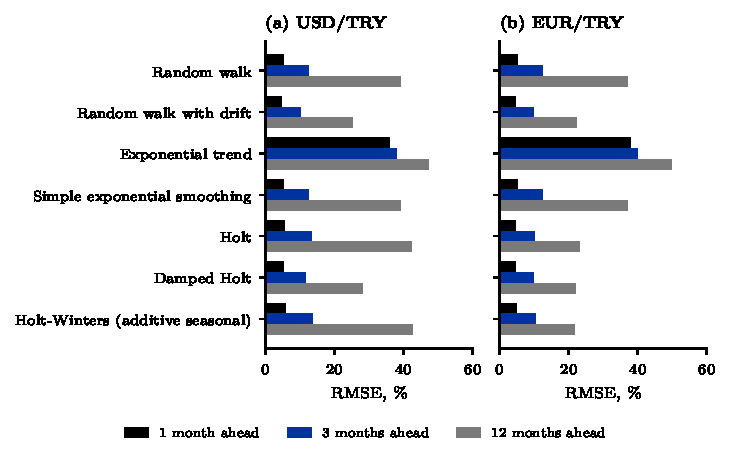
\includegraphics[width=\textwidth]{../figures/fig3_forecast.pdf}
\caption{RMSE of the forecasts on new months, by method and horizon.}
\end{figure}

\section{Conclusions and limitations}

\begin{enumerate}
\item The trend of USD/TRY and EUR/TRY is stochastic: a fixed exponential trend fits the past closely but forecasts poorly.
\item There is no monthly seasonality in the changes, so seasonal methods add nothing.
\item The random walk with drift is a hard benchmark: for USD it is the most accurate at every horizon, for EUR damped Holt and
Holt--Winters are within half a point of it.
\item Limitations: one evaluation window (2021--2026) that includes large depreciations; RMSE only; no test of the differences
between methods.
\end{enumerate}

\textbf{Scope and verification note.} Every number in this note is written by \texttt{make\_paper.py} from the CSV tables of the
analysis. \texttt{tests/run\_tests.py} checks the moving average, the trend regression, the seasonality tests and the forecasting
scheme against independent computations, and reproduces version 1's output ($R^2$ = 0.945 on its own data).

\section*{References}
{\small
\setlength{\parskip}{2pt}
\hangindent=1.27cm\hangafter=1 Durbin, J., \& Watson, G. S. (1951). Testing for serial correlation in least squares regression. II.
\textit{Biometrika}, 38(1/2), 159--177.\par
\hangindent=1.27cm\hangafter=1 Gardner, E. S., Jr., \& McKenzie, E. (1985). Forecasting trends in time series. \textit{Management Science},
31(10), 1237--1246.\par
\hangindent=1.27cm\hangafter=1 Holt, C. C. (2004). Forecasting seasonals and trends by exponentially weighted moving averages.
\textit{International Journal of Forecasting}, 20(1), 5--10.\par
\hangindent=1.27cm\hangafter=1 Hyndman, R. J., \& Athanasopoulos, G. (2021). \textit{Forecasting: Principles and practice} (3rd ed.). OTexts.\par
\hangindent=1.27cm\hangafter=1 Meese, R. A., \& Rogoff, K. (1983). Empirical exchange rate models of the seventies: Do they fit out of sample?
\textit{Journal of International Economics}, 14(1--2), 3--24.\par
\hangindent=1.27cm\hangafter=1 Winters, P. R. (1960). Forecasting sales by exponentially weighted moving averages. \textit{Management
Science}, 6(3), 324--342.\par
}
\end{document}
